\documentclass{article}
\usepackage[utf8]{inputenc}
\usepackage{graphicx}
\usepackage{titling}
\usepackage{pgfgantt}
\usepackage{pdflscape}
\usepackage{hyperref}
\usepackage{animate}
\usepackage{movie15}

\renewcommand{\refname}{Kaynakça}
\pretitle{
  \begin{center}
  \LARGE\bfseries
  
\includegraphics[width=0.1\textwidth]{logo.png} 
  \vskip 1em
  }
  \posttitle{
  \end{center}
}
\title{Yapay Zeka ile Görüntü Gürültüsü Azaltma Projesi}
\author{İlyas Cemal Erginli}
\date{Mart 2024}

\begin{document}
\begin{titlepage}
    \maketitle
    \begin{center} 
        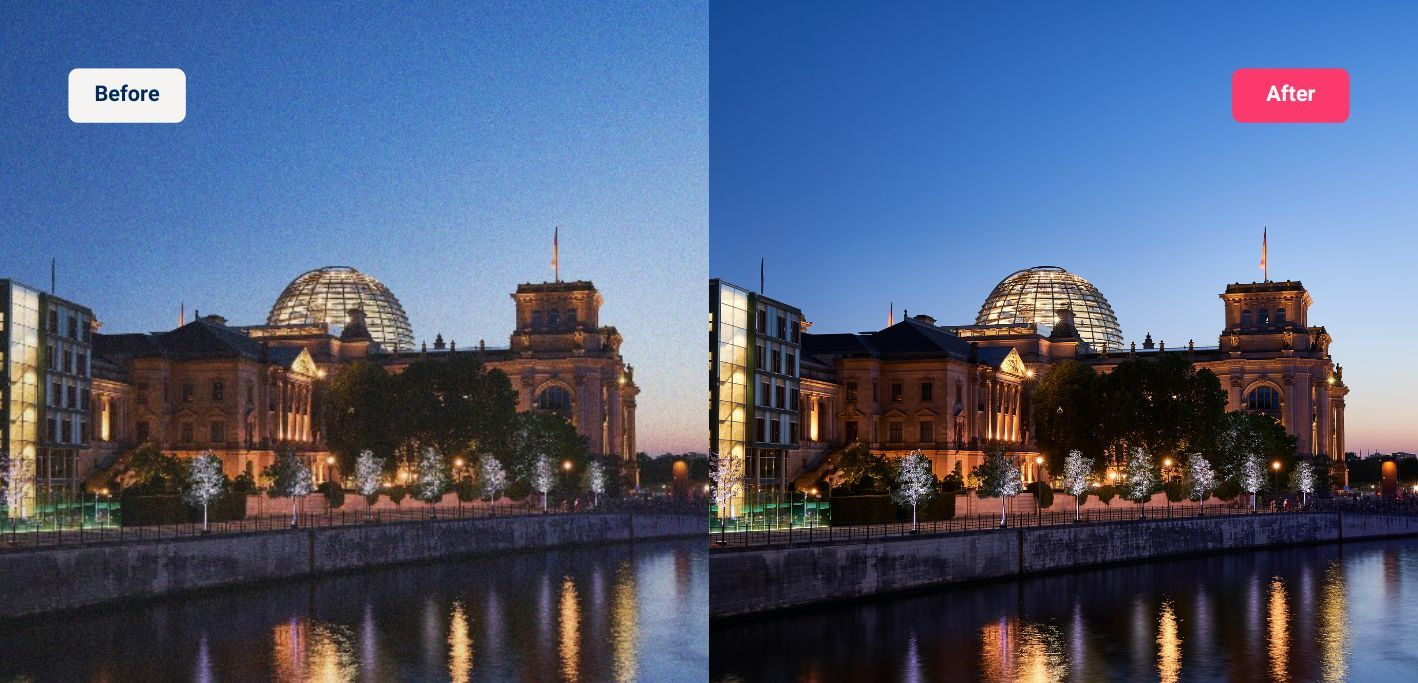
\includegraphics[width=0.8\textwidth]{imageAı.jpg}
    \end{center}
    \thispagestyle{empty}
    \vfill
    \rule{\textwidth}{0.5pt}
    \renewcommand{\abstractname}{Özet}
    \begin{abstract}
    \noindent Bu projenin amacı, gürültülü görüntülerdeki istenmeyen gürültüyü azaltarak veya ortadan kaldırarak daha net ve kaliteli görüntüler elde etmektir. Bu proje, çeşitli alanlarda (örneğin, tıbbi görüntüleme, fotoğrafçılık, video işleme) kullanılabilecek, gürültülü görüntülerin kullanışlılığını artırmayı hedefler. Yapay zeka modelleri, gürültülü görüntülerdeki desenleri ve yapıları tanıyarak gürültüyü azaltmak için öğrenilmiş bilgiyi kullanır. Bu proje, daha iyi görsel kalite ve daha doğru analiz sonuçları elde etmek için gürültülü görüntülerin iyileştirilmesine odaklanır.
    \end{abstract}
    \rule{\textwidth}{0.5pt}
    \vfill

\end{titlepage}
\newpage

\noindent \section{Giriş}
\rule{\textwidth}{0.5pt}\\[10pt]
Günümüzde, dijital görüntüleme teknolojileri hızla gelişmekte ve yaygın bir şekilde kullanılmaktadır. Ancak, bu teknolojilerin kullanımında sıkça karşılaşılan bir sorun da görüntülerin gürültülü olmasıdır. Gürültü, birçok faktörden kaynaklanabilir ve görüntülerin kalitesini düşürerek bilgi kaybına neden olabilir. Bu nedenle, görüntü gürültüsünün azaltılması, görüntüleme teknolojilerinin etkinliğini artırmak ve veri analizi süreçlerini iyileştirmek için önemli bir gerekliliktir. \\[10pt]

 \noindent Bu proje, yapay zeka tekniklerini kullanarak görüntü gürültüsünün azaltılmasını hedeflemektedir. Yapay zeka, özellikle derin öğrenme teknikleri, karmaşık veri yapılarını işleyebilme yetenekleriyle gürültü azaltma işlemlerinde etkili bir şekilde kullanılmaktadır. Bu proje kapsamında, gelişmiş yapay zeka algoritmaları ve derin öğrenme modelleri, gürültülü görüntülerin temizlenmesi için kullanılacak ve daha net ve kaliteli görüntüler elde edilmesi sağlanacaktır.\\[10pt]

\section{Literatür Çalışması}
\rule{\textwidth}{0.5pt}

 \noindent Bu makalede\cite{zhang2018ffdnet}, Hızlı ve etkili bir görüntü gürültü giderme yöntemi olan FFDNet, ayırt edici öğrenme yöntemlerinden farklı olarak geniş bir gürültü seviyesi aralığını tek bir ağla ele alabilir. Esnek bir yapıya sahip olan FFDNet, giriş olarak ayarlanabilir bir gürültü seviye haritası kullanarak mekansal olarak değişken gürültüyü de çıkarabilir. Ayrıca, örnekleme yapılmış alt görüntüler üzerinde çalışarak hızlı çıkarım hızı sağlar ve BM3D'e kıyasla daha hızlı sonuçlar elde eder. Yapılan deneyler, FFDNet'in etkili ve verimli olduğunu göstermiştir, bu da pratik gürültü giderme uygulamaları için cazip bir seçenek haline getirir.\\[10pt]

 \noindent Bu makalede\cite{yu2019deep}, Düşük seviye görüş araştırmalarında yaygın olarak incelenen özellik haritalarının indirme ve yükleme ölçeklendirme kullanılarak ağlar, verimli GPU bellek kullanımı ve geniş duyarlı alanları sağlama kapasiteleri nedeniyle incelenmiştir. Bu bağlamda, görüntü gürültü giderme için derin tekrarlayan indirme-yükleme evrişimli sinir ağı (DIDN) önerilmektedir. Bu ağ, özellik haritalarının çözünürlüğünü tekrar tekrar azaltıp artırır. Ağın temel yapısı, özgün olarak anlamsal segmentasyon için geliştirilen U-Net'ten esinlenmiştir. İndirme ve yükleme katmanları, görüntü gürültü giderme görevi için uyarlanmıştır. Geleneksel gürültü giderme ağları, tek seviyeli gürültüyle çalışması için eğitilmiştir veya alternatif olarak, tek bir modelle çoklu seviyeli gürültüyü ele almak için gürültü bilgisini giriş olarak kullanır. Bununla birlikte, ağımızın etkili bellek kullanımı, tek bir modelle gürültünün geniş bir aralığını işlemesini sağlar ve bu da gürültü bilgisi girişlerine ihtiyaç duymadan çoklu seviyeli gürültüyü ele almasını sağlar.\\[10pt]


\noindent
\section{Yöntemler}
\rule{\textwidth}{0.5pt}
Bu projede, Convolutional Neural Network (CNN) gibi derin öğrenme yöntemleri yanı sıra, temiz veri oluşturma için kullanılan autoencoder gibi unsupervised öğrenme teknikleri de kullanılacaktır. Autoencoder'lar, gürültülü görüntüyü giriş olarak alıp, gizli katmanlarda temiz görüntüyü oluşturarak gürültü azaltma sürecini gerçekleştirirler. Ayrıca, gürültülü görüntülerdeki istenmeyen özelliklerin tanımlanması için denetimli öğrenme yöntemleri de uygulanabilir. Bu yöntemlerde, gürültülü ve temiz görüntülerin eşleştirildiği bir eğitim veri seti kullanılarak, gürültülü görüntülerden temiz görüntülerin tahmini için öğrenme gerçekleştirilir.\\[10pt]

 \noindent Bu farklı yöntemlerin kombinasyonu, gürültü azaltma sürecindeki etkinliği artırabilir ve çeşitli gürültü tipleriyle başa çıkabilme kabiliyetini sağlayabilir. Autoencoder'lar, gürültülü verilerden temiz verilerin oluşturulmasında kullanılarak, CNN'lerin daha iyi performans göstermesine yardımcı olabilir. Denetimli öğrenme yöntemleri ise belirli gürültü tiplerine özgü özelliklerin tanımlanması ve gürültü azaltma işleminin hassaslaştırılması için önemli bir rol oynar. Bu yöntemlerin bir araya getirilmesi, daha güçlü ve esnek bir gürültü azaltma çözümü elde etmek için önemlidir.\\[10pt]


\section{Modeller}
\begin{enumerate}
    \item Autoencoder
    \item FFDNet(Feedforward Neural Network)
    \item DnCNN(Denoising Convolutional Neural Network)
    
\end{enumerate}

\newpage
\subsection{Aoutoencoders}

\noindent Aoutoencoderlar, görüntüler, vektörler, ses veya buna benzer bir tür giriş verisi alan ve önce orijinal giriş verilerini daha düşük bir boyuta sıkıştıran ve ardından verilerin bu daha düşük boyutlu temsilini kullanan bir tür yapay sinir ağıdır.
Eğitim süreci boyunca, kayıp fonksiyonu kullanılarak encoder ve decoder ağlarındaki parametreler ayarlanır. Bu ayarlamalar, encoder ve decoder'ın veriyi sıkıştırma ve tekrar oluşturma yeteneklerini geliştirir.\vspace{1 cm}

Mean Squared Error (MSE) 
\begin{equation}
    \frac{1}{n} \sum_{i=1}^{n} (x_{i} - \hat{x}_{i})^2
\end{equation}

Mean Absolute Error (MAE)
\begin{equation}
    \frac{1}{n} \sum_{i=1}^{n} |x_{i} - \hat{x}_{i}|
\end{equation}

\renewcommand{\figurename}{Şekil}

\begin{figure}[htbp]
     \centering
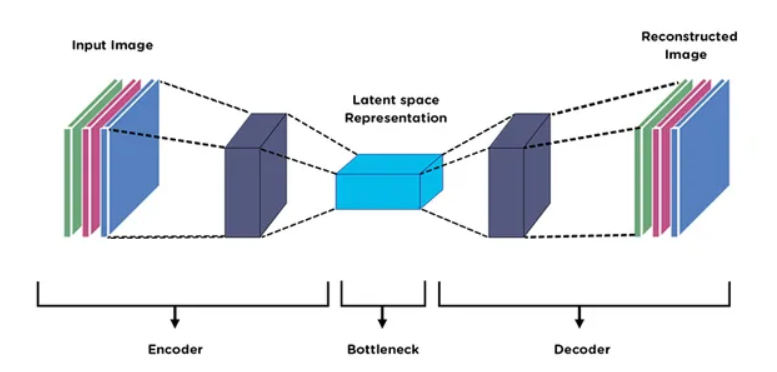
\includegraphics[angle=360,width=1.1\textwidth]{autoencoder.png}\centering 
  \caption{Aoutoencoder\cite{Autoencoder}}
  \label{fig:resim_etiketi}
\end{figure}

\newpage
\subsection{FFDNet}

\noindent Giriş görüntüsü alt görüntüler halinde yeniden şekillendirilir ve bunlar daha sonra bir gürültü seviyesi haritasıyla birlikte CNN’e girilir. Nihai çıktı, gürültüden arındırılmış alt görüntüler tarafından yeniden oluşturulur. Bu modelde de kayıp fonksiyonu kullanılır.
\vspace{1 cm}

Mean Squared Error (MSE) 
\begin{equation}
    \frac{1}{n} \sum_{i=1}^{n} (x_{i} - \hat{x}_{i})^2
\end{equation}

\renewcommand{\figurename}{Şekil}

\begin{figure}[htbp]
     \centering
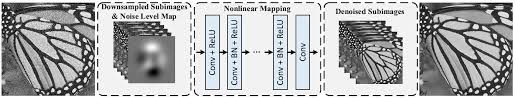
\includegraphics[angle=360,width=1.1\textwidth]{ffdnet.jpeg}\centering 
  \caption{FFDNet\cite{zhang2018ffdnet}}
  \label{fig:resim_etiketi}
\end{figure}

\subsection{DnCNN}

\noindent DnCNN, bir dizi evrişim katmanı, ReLU aktivasyon fonksiyonları ve gürültü azaltma amacıyla tasarlanmış özel bir eğitim kaybı fonksiyonunu içerir. Evrişim katmanları, görüntüdeki özellikleri çıkarmak ve öğrenmek için kullanılırken, ReLU aktivasyon fonksiyonları ağın doğrusallığı kırarak daha karmaşık özellikleri öğrenmesine yardımcı olur. Eğitim süreci boyunca, ağ gürültülü görüntüler ile temiz görüntüler arasındaki farkı minimize etmeyi öğrenir. Bu modelde de kayıp fonksiyonu kullanılır.\vspace{1 cm}

Mean Squared Error (MSE) 
\begin{equation}
    \frac{1}{n} \sum_{i=1}^{n} (x_{i} - \hat{x}_{i})^2
\end{equation}

\renewcommand{\figurename}{Şekil}

\begin{figure}[htbp]
     \centering
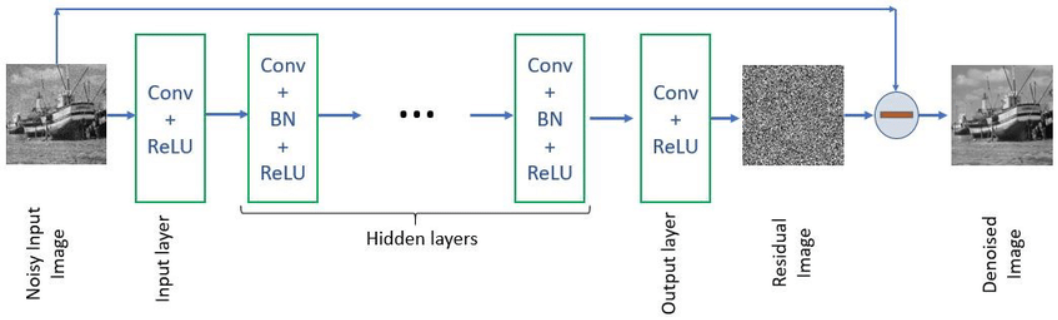
\includegraphics[angle=360,width=1.1\textwidth]{dncnn.png}\centering 
  \caption{FFDNet\cite{alawode2021dense}}
  \label{fig:resim_etiketi}
\end{figure}
\newpage

\section{Veri Setinin Oluşturulması}
\rule{\textwidth}{0.5pt}\\[10pt]

 \noindent Bu hafta, Pexels\cite{Pexels} ve Pixabay\cite{Pixabay} gibi web sitelerinden farklı türlerde toplam 100 görsel indirdim. Ardından bu görsellere 4 farklı gürültü ekleme algoritması uyguladım: Gauss gürültüsü, salt and pepper gürültüsü, Gauss and SP gürültüsü, ve Gauss bulanıklığı. Bu işlemlerin sonucunda toplamda 400 farklı çıktı elde ettim. Bu çıktılar sayesinde veri setimi oluşturmuş oldum. Görselleri indirmek için Pexels ve Pixabay gibi platformları tercih ettim çünkü bu siteler geniş bir görsel koleksiyonuna sahiptir ve farklı kategorilerde görsellere erişim sağlarlar. Bu çeşitlilik, veri setimin çeşitliliğini artırmama yardımcı oldu. Bu süreçte farklı gürültü türlerini anlamak ve bu gürültülerin görüntüler üzerindeki etkilerini gözlemlemek de önemli bir deneyim oldu.\vspace{0,5cm}

\noindent Ardından, her görsel üzerine farklı gürültü eklemek için 4 farklı algoritma kullandım:\vspace{0,5cm}

\noindent Gauss Gürültüsü: Bu algoritma\cite{Github}, pikseller üzerinde gauss dağılımına göre rastgele değerler ekler, böylece görselde yumuşak bir gürültü efekti oluşturur.\vspace{0,5cm}

\noindent Salt and Pepper Gürültüsü: Bu algoritma\cite{Github2}, piksellerin bazılarını siyah-beyaz veya beyaz-siyah olarak değiştirerek görselde noktasal bir gürültü oluşturur.\vspace{0,5cm}

\noindent Gauss and SP Gürültüsü: Bu algoritma, gauss ve salt-and-pepper gürültülerini birleştirir, böylece hem gauss gürültü hem de noktasal gürültü efekti elde edilir.\vspace{0,5cm}

\noindent Gauss Bulanıklığı: Bu algoritma\cite{OpenCV}, görselde bulanıklık yaratır ve keskin kenarları yumuşatır.\vspace{0,5cm}

%\section{Gauss Gürültüsü}
\begin{figure}
     \centering
 \noindent 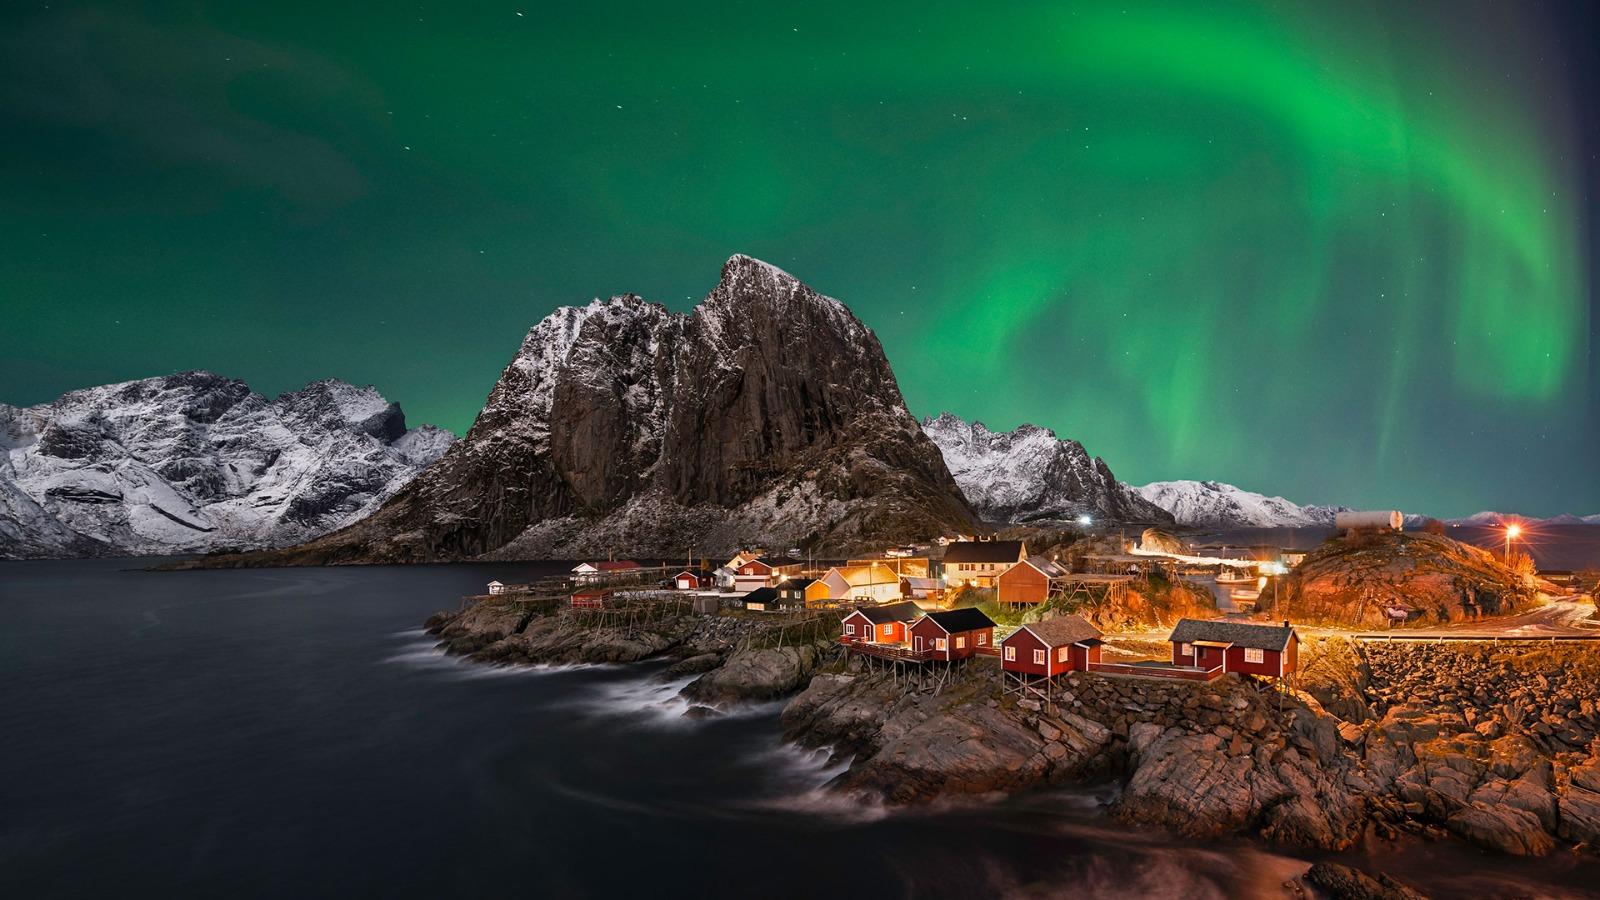
\includegraphics[angle=360,width=1.1\textwidth]{9.jpg}\centering 
  \caption{Orijinal Görsel}
  \label{fig:resim_etiketi}
\end{figure}

%\section{Gauss Gürültüsü}
\begin{figure}
     \centering
 \noindent 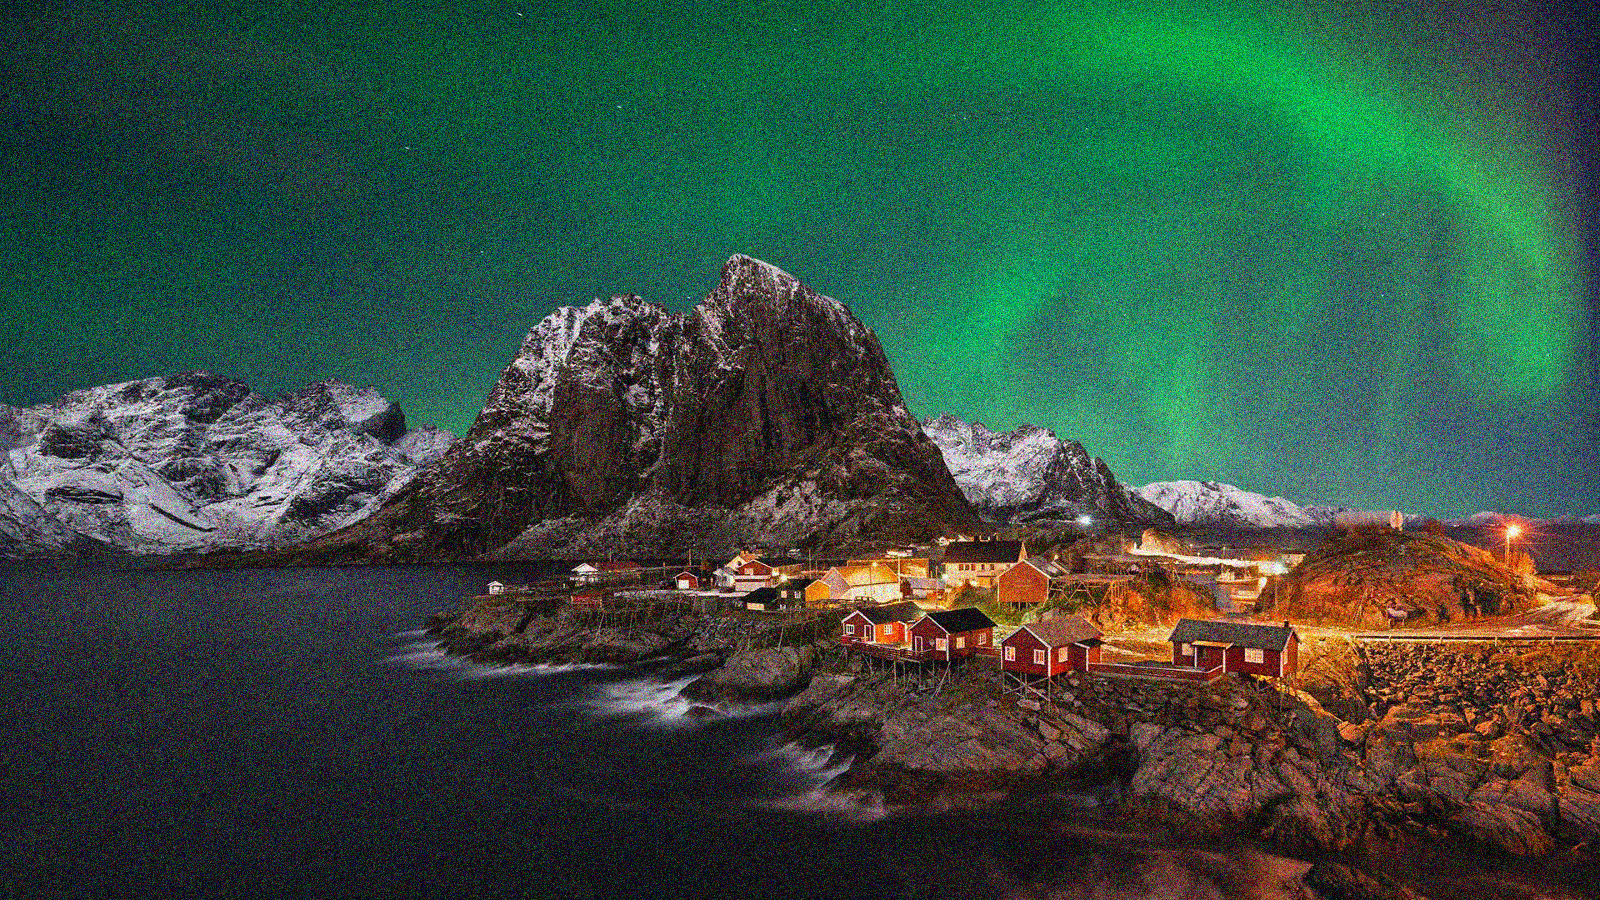
\includegraphics[angle=360,width=1.1\textwidth]{GaussN.png}\centering 
  \caption{Gauss Gürültüsü}
  \label{fig:resim_etiketi}
\end{figure}


%\section{Salt and Pepper Gürültüsü}
\begin{figure}
     \centering
  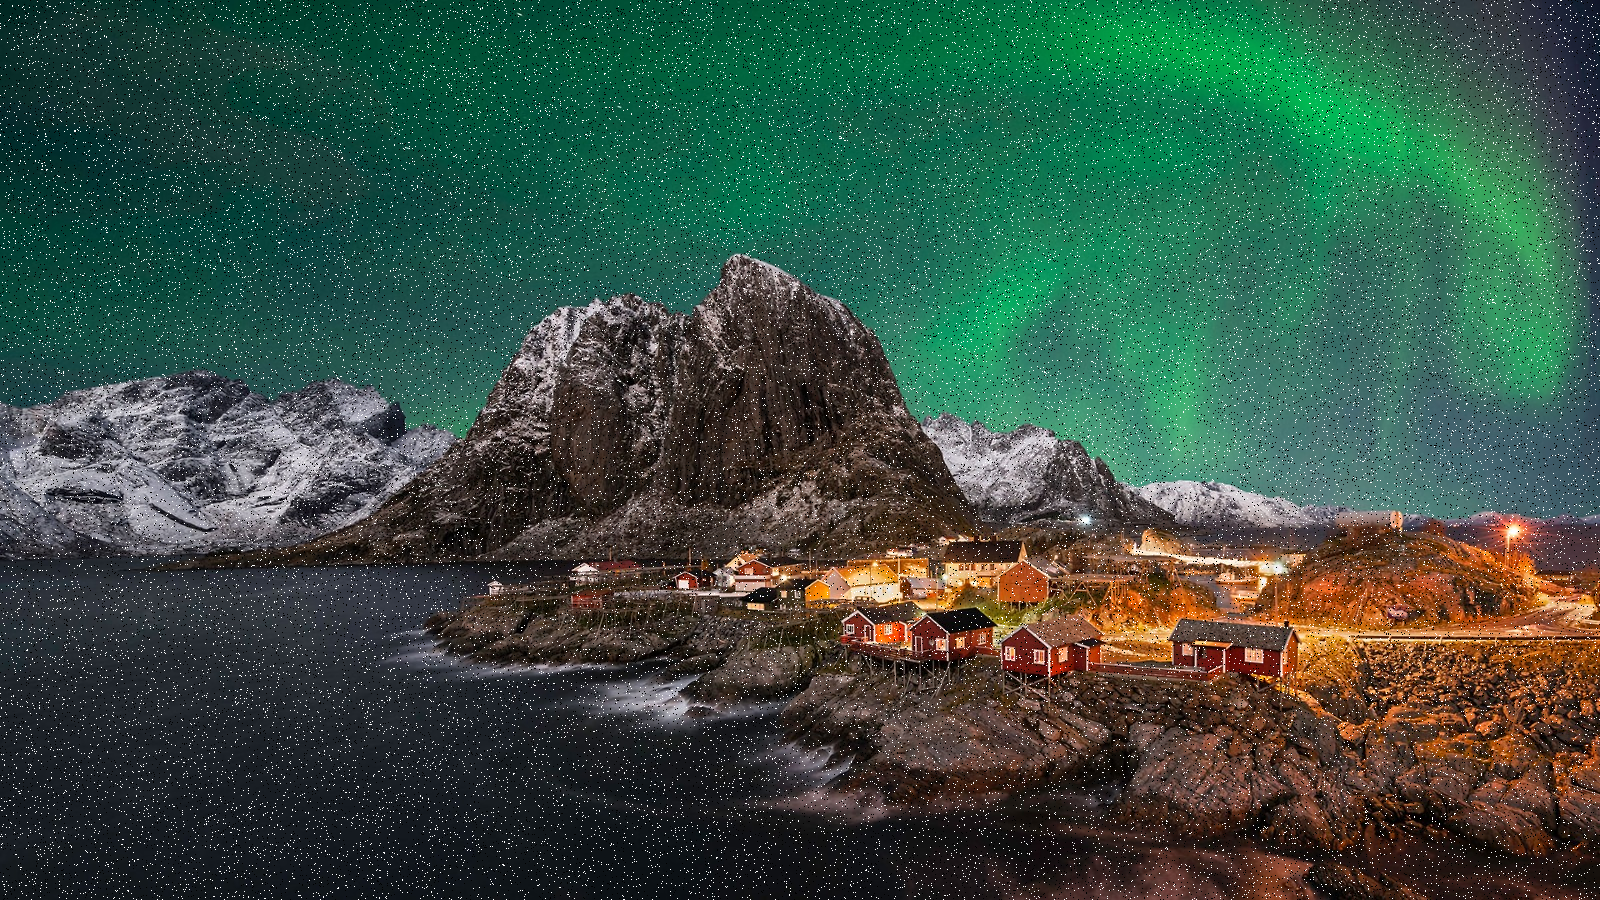
\includegraphics[angle=360,width=1.1\textwidth]{SPN.png}\centering 
  \caption{Salt and Pepper Gürültüsü}
  \label{fig:resim_etiketi}
\end{figure}

%\section{Gauss and SP Gürültüsü}
\begin{figure}
     \centering
  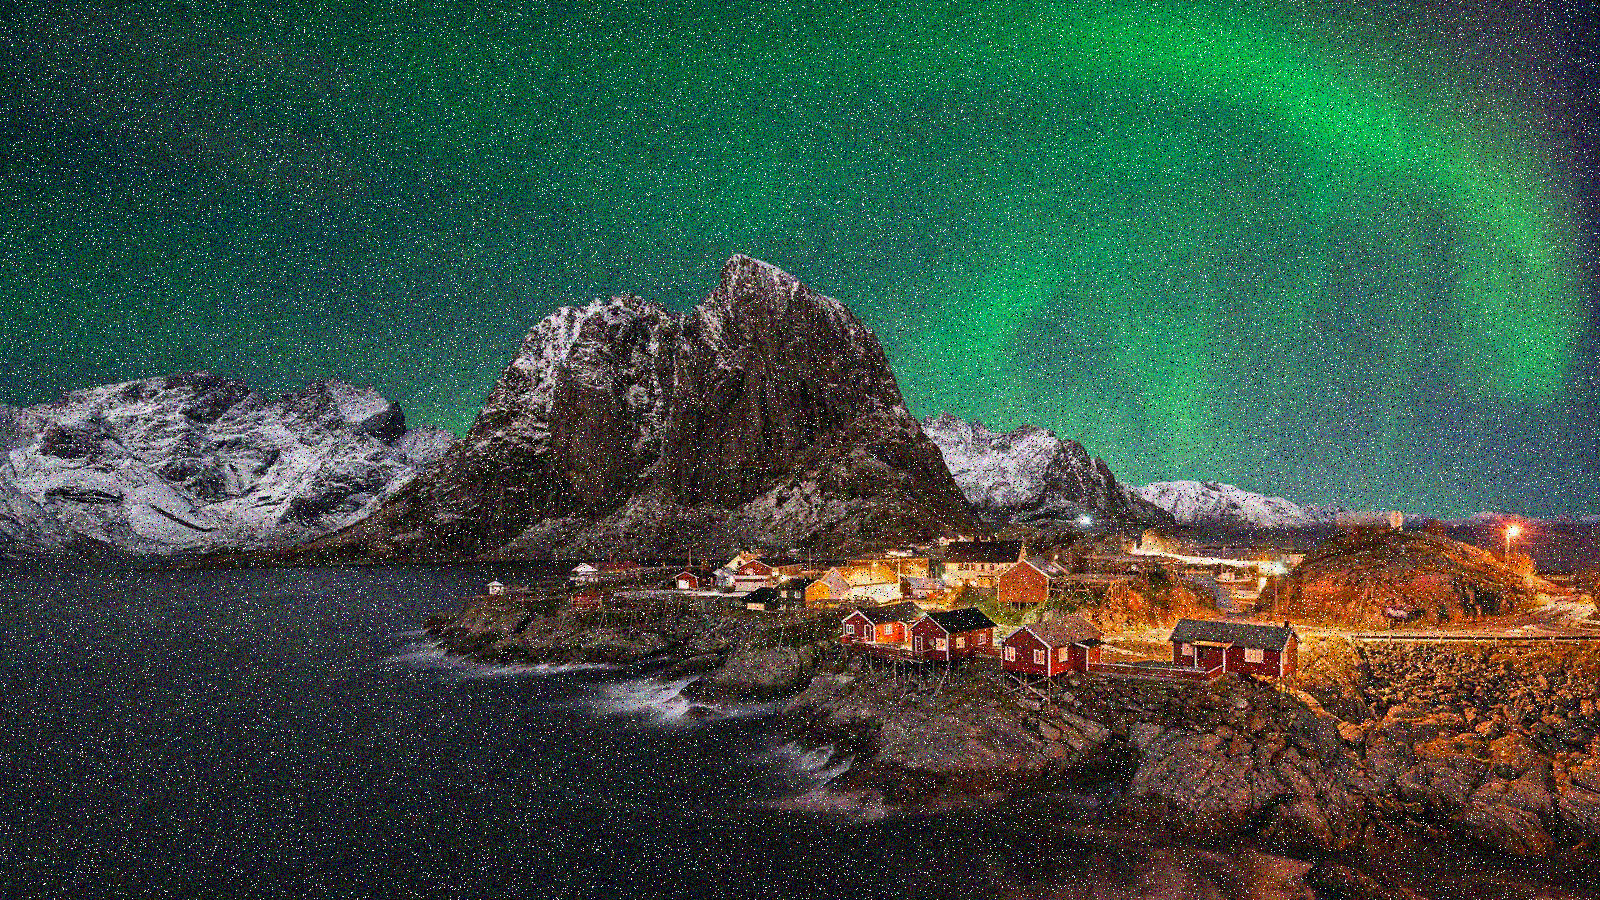
\includegraphics[angle=360,width=1.1\textwidth]{GaussAndSPN.png}\centering 
  \caption{Gauss and SP Gürültüsü}
  \label{fig:resim_etiketi}
\end{figure}

%\section{Gauss Bulanıklığı Gürültüsü}
\begin{figure}
     \centering
  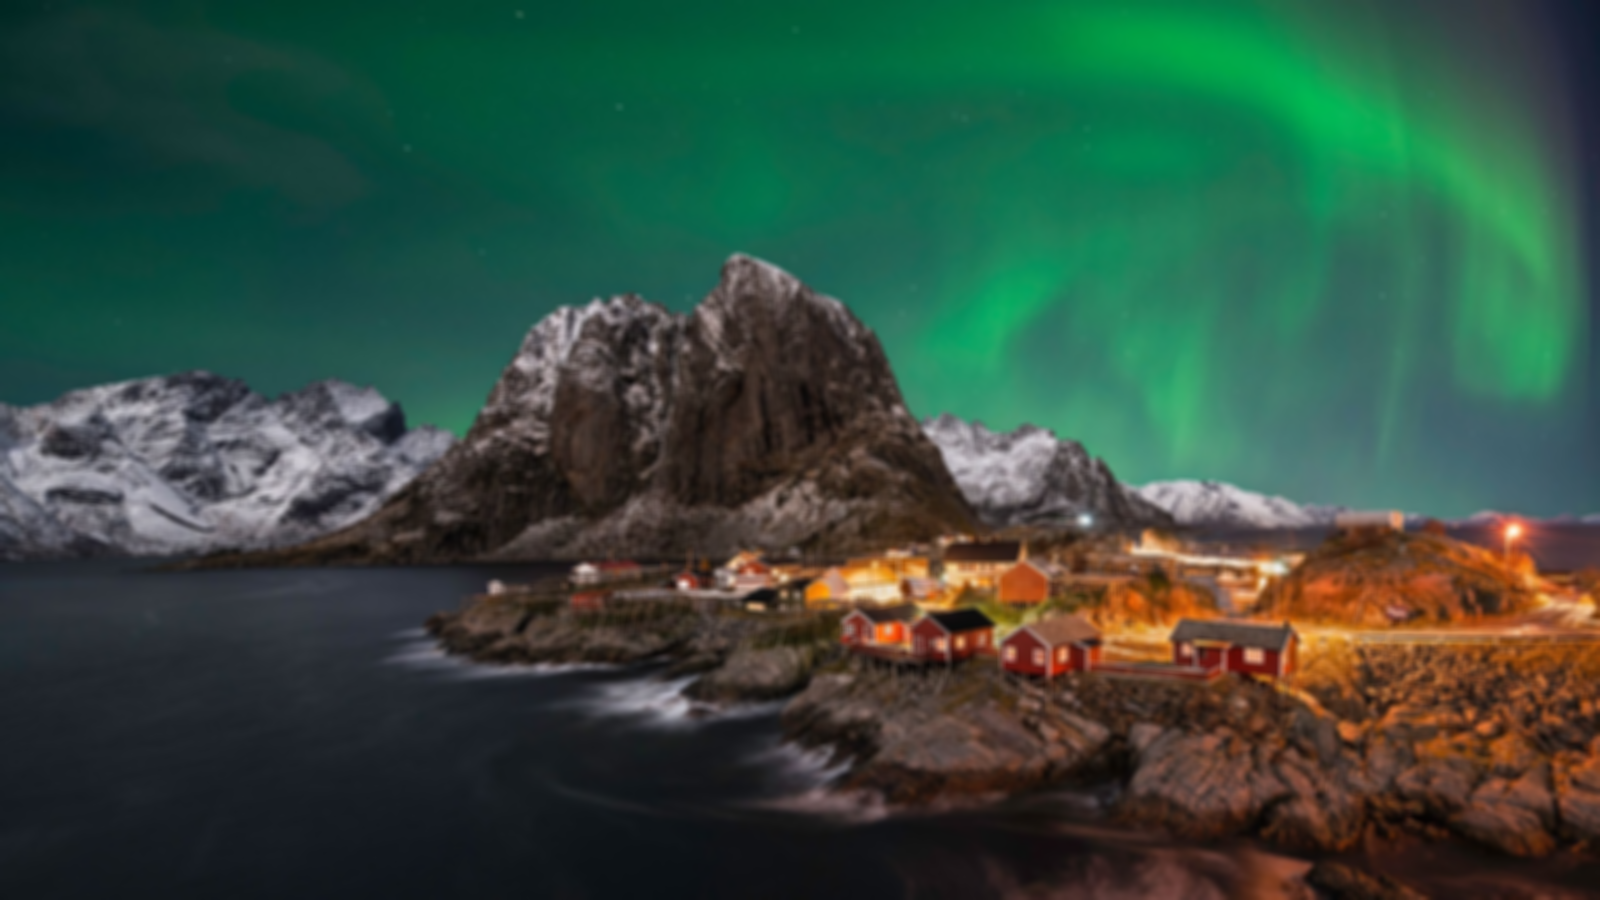
\includegraphics[angle=360,width=1.1\textwidth]{GaussBulanıklıgı.png}\centering 
  \caption{Gauss Bulanıklığı Gürültüsü}
  \label{fig:resim_etiketi}
\end{figure}

\newpage
\noindent Gösterdiğim algoritmaları kullanarak elde ettiğim görselleri gürültü türüne göre sınıflandırdım.\vspace{0,5cm}

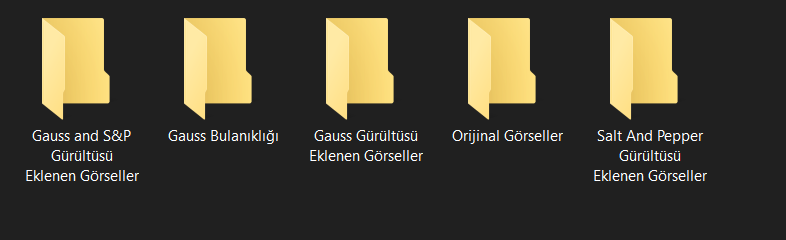
\includegraphics[width=1\textwidth]{Sınıflandırma.png}\vspace{0,5cm}

\newpage
\section{Yapay Zeka Oluşturulması}
\rule{\textwidth}{0.5pt}\\[10pt]

\noindent Bu hafta, bu projenin önceden yapılmış örneklerine\cite{Github3} bakarak yapacağım modelin nasıl yapılacağını, kodları anlayarak kendi projemde nelerin kullanılacağını ve kodlamamımı nasıl yapacağımı öğrenerek örnek projeler oluşturdum.\vspace{0.5cm}

\noindent Öncelikle yaptığım örnekler için hazır veri setleri kullandım. Bu örnekleri geliştirerek yapacağım asıl projede kendi veri setimi kullanacağım. Bu örneklerde hazır veri seti kullanmamın nedeni veri setindeki verilerin boyutunun aynı ve küçük olmasıdır. Böylece daha hızlı eğitimler yaparak kodların işlevselliğini hızlı bir şekilde kontrol edebilirim. Şu anki amacım kodları ve mantığını öğrenmek olduğu için örneklerimde bu veri setlerini kullandım.\vspace{0.5cm}

\noindent İlk oluşturduğum örnek için MNIST(Modified National Institute of Standards and Technology Database) veri setini kullandım. Bu veri seti 28x28 boyutunda, el yazısı rakamlardan oluşan siyah-beyaz bir veri setidir.\vspace{0.5cm}

\noindent İkinci oluşturduğum örnek için CIFAR-10(Canadian Institute For Advanced Research) veri setini kullandım. Bu veri seti 32x32 boyutunda gündelik hayattan pek çok görsel içeren,10 farklı sınıftan oluşan renkli bir veri setidir\vspace{0.5cm}

\noindent İki örneğin de kayıp fonksiyonlarıyla kayıp oranlarını grafikleştirdim. \vspace{0.5cm}

\renewcommand{\figurename}{Şekil}

\begin{figure}[htbp]
     \centering
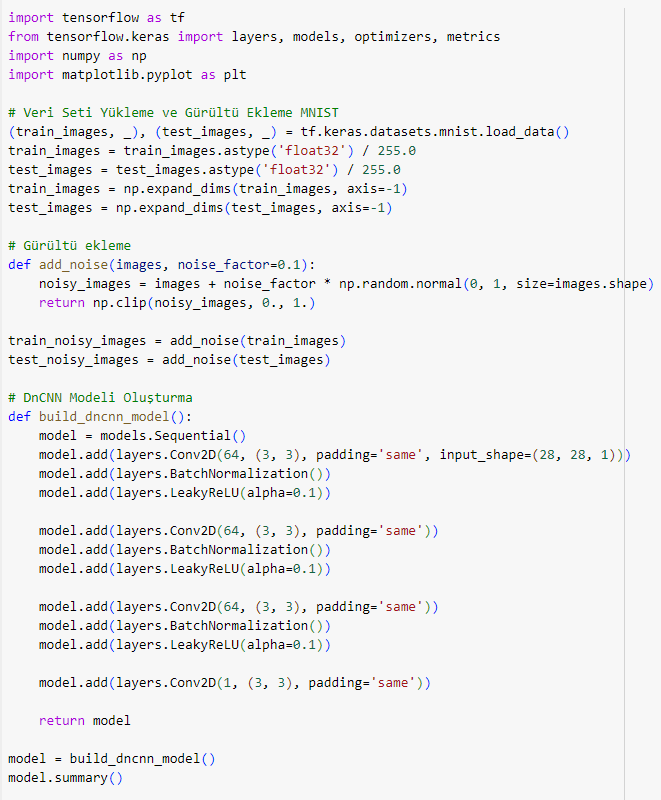
\includegraphics[angle=360,width=1.1\textwidth]{mnıst1.png}\centering 
  \caption{Kod}
  \label{fig:resim_etiketi}
\end{figure}

\renewcommand{\figurename}{Şekil}

\begin{figure}[htbp]
     \centering
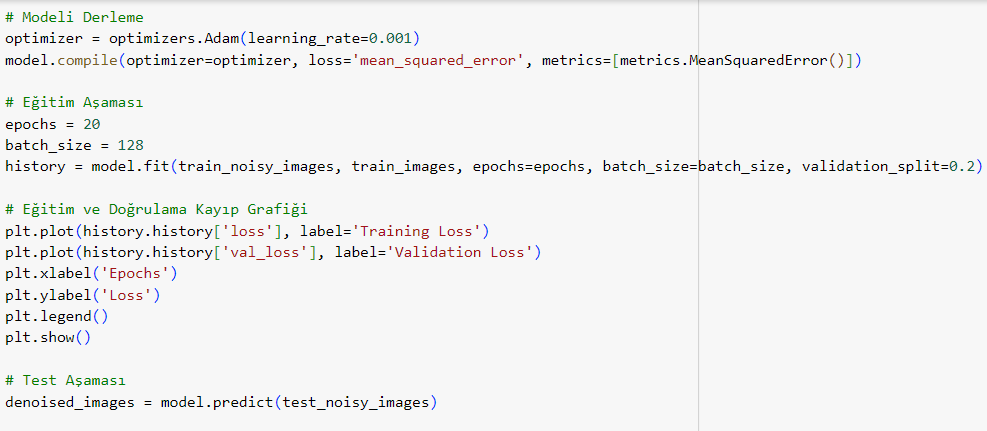
\includegraphics[angle=360,width=1.1\textwidth]{mnıst2.png}\centering 
  \caption{Kod}
  \label{fig:resim_etiketi}
\end{figure}

\renewcommand{\figurename}{Şekil}

\begin{figure}[htbp]
     \centering
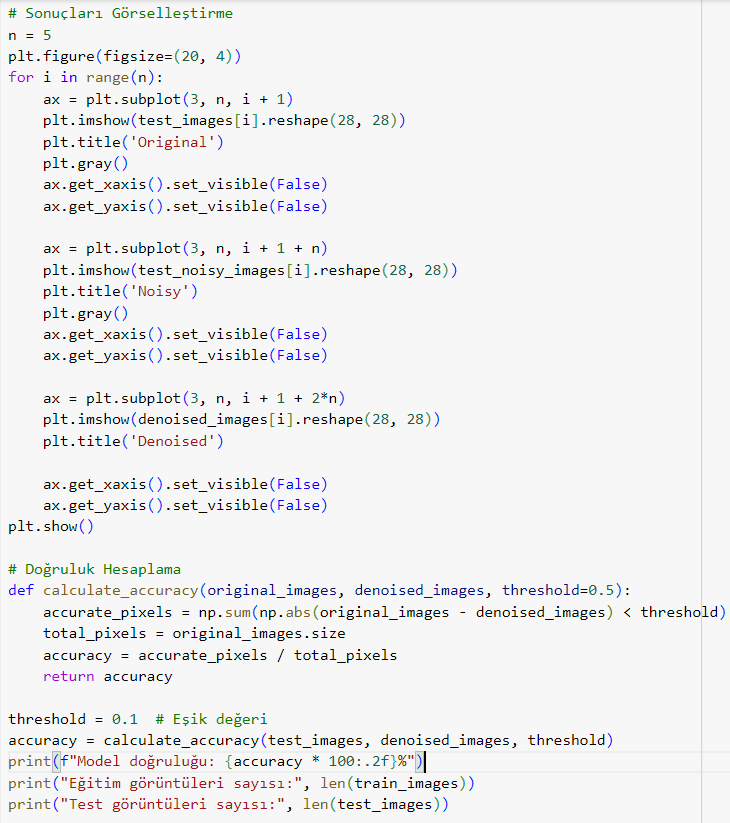
\includegraphics[angle=360,width=1.1\textwidth]{Mnıst3.png}\centering 
  \caption{Kod}
  \label{fig:resim_etiketi}
\end{figure}


\clearpage
\noindent Epoch sayılarına göre başarı oranları değişmektedir.

\renewcommand{\figurename}{Şekil}

\begin{figure}[htbp]
     \centering
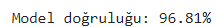
\includegraphics[angle=360,width=1\textwidth]{20epoch.png}\centering 
  \caption{Epoch=20 ise}
  \label{fig:resim_etiketi}
\end{figure}

\renewcommand{\figurename}{Şekil}

\begin{figure}[htbp]
     \centering
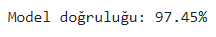
\includegraphics[angle=360,width=1\textwidth]{50epoch.png}\centering 
  \caption{Epoch=50 ise}
  \label{fig:resim_etiketi}
\end{figure}

\renewcommand{\figurename}{Şekil}

\begin{figure}[htbp]
     \centering
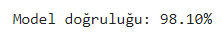
\includegraphics[angle=360,width=1\textwidth]{100epoch.png}\centering 
  \caption{Epoch=100 ise}
  \label{fig:resim_etiketi}
\end{figure}

\clearpage
\noindent İki örneğin de kayıp fonksiyonlarıyla kayıp oranlarını grafikleştirdim. \vspace{0.5cm}

\renewcommand{\figurename}{Şekil}

\begin{figure}[htbp]
     \centering
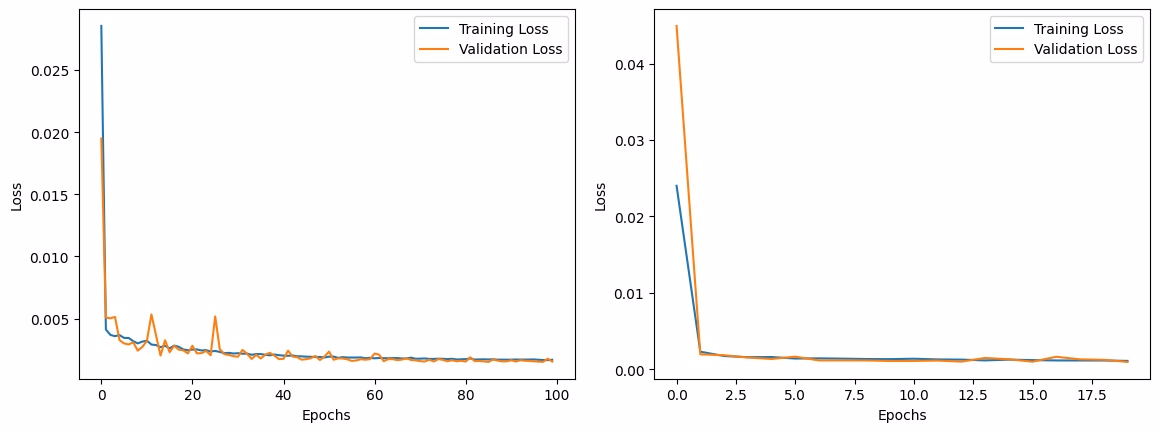
\includegraphics[angle=360,width=1\textwidth]{yz3(4).jpg}\centering 
  \caption{Kayıp Grafikleri}
  \label{fig:resim_etiketi}
\end{figure}



\noindent Burada yapmış olduğum 2 örneğin sonuçlarını göreceksiniz. \vspace{0.5 cm}


\begin{figure}[htbp]
     \centering
 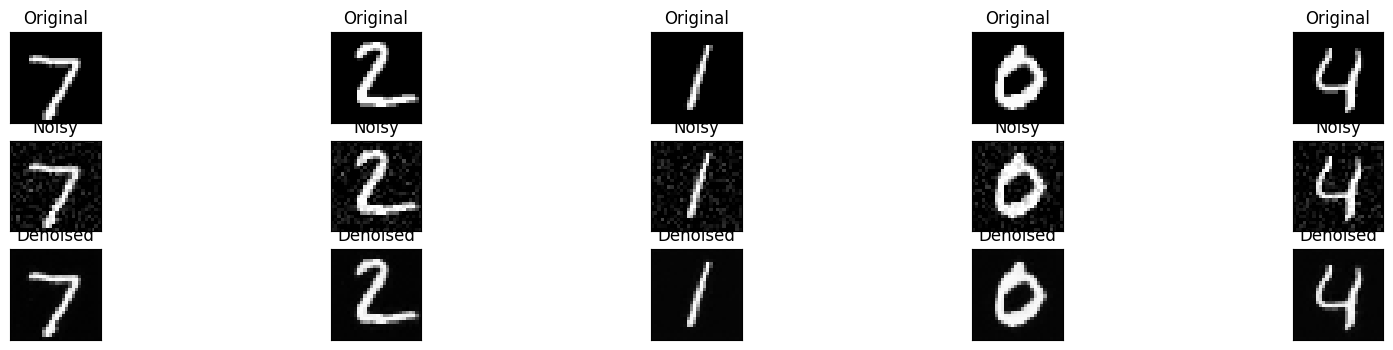
\includegraphics[angle=360,width=1\textwidth]{yz3.png}\centering 
  \caption{İlk Örneğin Sonucu}
  \label{fig:resim_etiketi}
\end{figure} \vspace{1 cm}


\begin{figure}[htbp]
     \centering
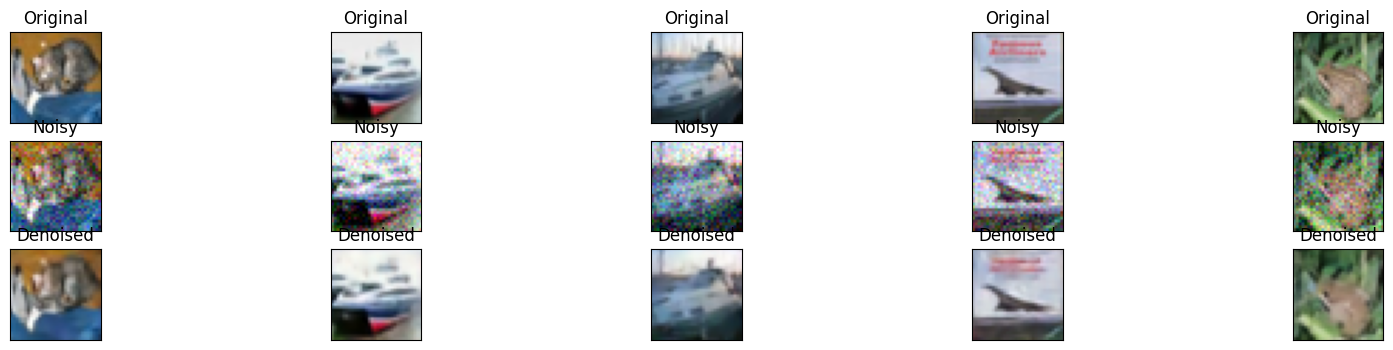
\includegraphics[angle=360,width=1\textwidth]{yz3(1).png}\centering 
  \caption{İkinci Örneğin Sonucu}
  \label{fig:resim_etiketi}
\end{figure}

\clearpage
\newpage

\bibliographystyle{ieeetr}
\bibliography{ref3}

\end{document}